\section{Analysis} \label{sec:analysis}
\subsection{Omnidirectional Exchange Model}
%
This section investigates the benefits of a unicurrency LP protocol. It addresses precisely how network effects form and why businesses can benefit from integrating their LPs into a protocol that promotes loyalty partnerships and increased redemption options. The following analysis combines insights from extant research to gain a comprehensive understanding of why the Koalition protocol enables a rich and interoperable LP ecosystem. Bolden \etal\ in \cite{Bolden14} argues that LPs derive their value from three inherent program characteristics: loyalty margin (LM), incremental share (IS), and program size. LM is defined as the difference between the perceived value of redeemed benefits to customers and the cost to the company for realizing those benefits. IS measures how the LP influences customer spending behavior-- it is the difference between total customer expenditure after the introduction of a LP and total customer expenditure beforehand. Lastly, program size is the share of the businesses' revenue generated from the LP. Goel's work in \cite{Goel17} introduces the notion of merchant utility and social welfare in coalition LPs. Using a bilateral negotiation model, Goel provides insight on how companies can optimally set their exchange rates with respect to these measures. In order to develop a unicurrency LP protocol, it is necessary adopt a model which eliminates exchange rates and accounts for the incremental utility of additional merchants to existing partners. %but preserve the original definitions of utility and social welfare. 

To develop this model, it is important to understand how two merchants benefit from a joint program. In this scenario, merchant $i$ and merchant $j$ have a loyalty partnership where type-$j$ customers (merchant $j$'s loyal customers) wish to avail services from merchant $i$-- type-$j$ customers are more likely to visit merchant $i$ if they are able to collect points at $i$ to redeem at merchant $j$. This excess demand is beneficial for merchant $i$ because it brings in immediate revenue from type-$j$ customers as well as future revenue from these new customers who may prefer merchant $i$ over its competitors in the future. Merchant $i$ also gains immediate revenue from type-$i$ customers redeeming points at merchant $i$, collected from merchant $j$. This is because merchant $i$ receives immediate revenue from the points redeemed since these points have market value. Merchant $i$ also continues to obtain immediate revenue from type-$i$ customers who collect and redeem points at merchant $i$ as if it were a stand-alone LP. On the other hand, every type-$i$ customer visit to merchant $j$ may result in a loss of immediate/future revenue to merchant $i$. This loss is greater with a more competitive merchant $j$, but is negligible if merchant $j$ provides a complimentary service. Lastly, merchant $i$ incurs a redemption cost for every point redeemed by type-$i$ and type-$j$ customers. \textbf{Might be worth to make an image of this}

First, define $\theta_{ij}$ as the rate of type-$i$ customers collecting points at merchant $j$ with the intention of redeeming them at merchant $i$. Next, $c_{ij} \in [0, 1]$ is a measure of the competitiveness between merchant $i$ and $j$ and is symmetric, \ie\ $c_{ij} = c_{ji}$. Next, the customer acquisition value, $a_i \geq 0$, represents the value the merchant obtains per point earned and converted by a type-$j$ customer. Again, this can be interpreted as the combination of immediate and future revenue from type-$j$ customers. Lastly, $q_i$ is defined as the difference between the market value per point redeemed and the cost to the merchant per point redeemed. Note that the market value per point redeemed is equivalent to the customer's perceived value per point, which makes $q_i$ exactly equivalent to the LM, as defined earlier. 

Given the above, the two-merchant utility for $i$ is
%
\begin{align*}
u_i = \theta_{ii}q_i + \pi_{ij}
\end{align*}
%
where $\pi_{ij}$ represents the incremental utility gained from merchant $i$ and $j$ establishing a loyalty partnership and is defined as
\begin{align*}
\pi_{ij} = \theta_{ji}a_i - \theta_{ij}(a_j c_{ij} - q_i)
\end{align*}
%
\textit{Social welfare} (\ie\ sum of incremental utilities) between merchants $i$ and $j$ is defined as
\begin{align*}
\pi_{ij} + \pi_{ji} = \theta_{ij}(a_j(1-c_{ij}) + q_i) + \theta_{ji}(a_i(1-c_{ji}) + q_j)
\end{align*}
Notice that social welfare is maximized when $c_{ij} = c_{ji} = 0$. Thus, It seems that loyalty partnerships that are the most beneficial are between two merchants that provide complementary services. All else equal, as the two merchants become more competitive (\ie, $c_{ij} > 0$), social welfare decreases. While social welfare decreases with increased competition, an environment where merchants offer substitutable services may cause type-$j$ customers to become type-$i$ customers (and vice versa). This is reflected as an increase in $\theta_{ii}$ (or $\theta_{jj}$) and so while social welfare decreases, individual utility, $u_i$ ($u_j$), may increase at the cost of merchant $j$ (merchant $i$). 

For the general case, the $N$-merchant utility for $i$ is
\begin{align*}
u_i = \theta_{ii}q_i + \Pi_i
\end{align*}
%
where $\Pi_i$ is the \textit{incremental network utility} and is defined as
\begin{align*}
\Pi_i & = \pi_{i1} + \pi_{i2} + \pi_{i3} + ... + \pi_{i(N-1)} + \pi_{iN} \\
& = \sum_{k=1}^N \big[\theta_{ki}a_i - \theta_{ik}(a_k c_{ik} - q_i) \big]
\end{align*}
%
Note that as $q_i$ (LM) increases, individual and incremental network utility increase. The general form of social welfare for $N$-merchants follows from the above definitions and is defined below. Note that the effect of non-competition for the two-merchant case generalizes to the $N$-merchant case, \ie\ $c_{ik} = 0$ for all $i, k \in \{1,...,N\}$ and $i \neq k$ maximizes social welfare. 
\begin{align*}
\Pi_1+ \Pi_2 + ... + \Pi_{N-1} + \Pi_N = \sum_{i=1}^N \sum_{k=1}^N \big[\theta_{ki}a_i - \theta_{ik}(a_k c_{ik} - q_i) \big]
\end{align*}
%
Furthermore, in the special case where all merchants provide complimentary services, $\Pi_i > 0$ for all $i \in \{1,...,N\}$ assuming $\sum_{k=1}^N\theta_{ki}$ and  $\sum_{k=1}^N\theta_{ik}$ are strictly positive and $q_i$ is non-negative. In other words, if competition between LPs is negligible in a protocol that permits customers to easily exchange their points among individual LPs with positive LMs, then merchants who join the protocol benefit because they gain additional customers. Also, since incremental network utility is positive for any given merchant, then as the number of merchants increases, social welfare also increases.

Next, we account for competition and determine under what LMs social welfare increases as the number of loyalty partnerships in the protocol grows. In order for social welfare to grow as $N$ grows, each additional merchant must have positive incremental network utility ($\ie\ \Pi_i > 0, \forall i \in \{1,...,N\}$). 
%
\footnote{Better to put condition in terms of LM?-- Need to find out: Do customers spend more money with more members in a coalition (this affect $a_i$)? Do they become more frequent visitors at any given merchant in a coalition? (this affects $\theta_{ij}$) Do they gain more "new" customers as coalition increases? (this affect $a_i$). Note lower $a_i$ is easier to obtain than a higher one since this means lower req'd change in customer behavior}
%
To achieve this condition, the LM ($q_i$) of any merchant $i$ must satisfy the following inequality:
\begin{align*}
q_i > \frac{\sum_{k=1}^N \theta_{ik} a_k c_{ik} - a_i \sum_{k=1}^N \theta_{ki}}{\sum_{k=1}^N \theta_{ik}}
\end{align*}
%
The first term of the numerator on right-hand side of the inequality is the \textit{total perceived cost of competition} to merchant $i$. The second term is the product of the total collection ratio and the customer acquisition value of merchant $i$, which is defined as the \textit{customer acquisition volume}.\footnote{come up with a more intuitive explanation of what this is and a good name that captures this product}

As the total perceived cost of competition to $i$ increases, merchant $i$'s LM must also increase to maintain positive incremental network utility (\ie\ continue to individually benefit from the network). This increased cost to merchant $i$ results from merchants on the protocol who offer substitutable services (increase $c_{ik}$) and are able to generate more immediate/future revenue merchant $i$'s loyal customers (increased $a_{k}$). One way to offset this increased cost from competition is to introduce \textit{switching costs} between competitive merchants. This serves as a barrier to discourage customers from availing services from a competitor and its effect can be interpreted as a decrease in $c_{ik}$. In the face of competition, switching cost can help merchants maintain a smaller LM but still achieve positive incremental network utility.  Lastly, for the special case of non-competitive merchants, the non-negativity assumption on $q_i$ (LM) can be relaxed. As long as the LM is greater than the negative of the customer acquisition volume, merchant $i$ is guaranteed to have positive incremental network utility. Note that this does not guarantee positive merchant utility (\ie\ $u_i > 0$) as the magnitude of the stand-alone LP utility may be greater than incremental network utility. Hence, while a merchant with a negative LM may still contribute to social welfare, it does not guarantee positive individual utility. 

On the other hand, as customer acquisition volume increases, the required LM to benefit on the network will decrease. This increase in volume can result from two things happening: 1) more ``new customers" collect points at merchant $i$ than customers leaving $i$ to collect from other merchants and 2) customers expend more at merchant $i$. This increase can essentially be attributed to an increase in the IS of a merchant's LP, hence it is necessary to show that as the number of merchants, $N$, increases, the LP's IS also increases (\ie\ the growth of the LP protocol leads to increased customer activity and spending). 

\subsection{Koalition LP Network}
%
According to \cite{Breu15}, there are two primary types of coalition LPs: \textit{dominant LP model} and \textit{equal-level partnership model}. In the former model, the dominant business runs the LP therefore communication and marketing revolves around the offerings of the dominant LP and is augmented by the offerings from the other partners. In the latter model, the coalition LP is typically run by a TTP specializing in LP management. Marketing efforts and communication towards customers are done through joint redemption promotions and increased redemption options. Using the omniexchange model developed in the last section, this section compares the \textit{utility} of these two types of coalition LP designs on the Koalition protocol. Specifically, it is shown that if individual merchant LPs can achieve a high enough LM, the equal-level partnership model promotes greater individual utility and social welfare compared to the dominant LP model. Furthermore, this section introduces the notion of switching costs in the form of fees when redeeming points between two directly competing firms. For example, in order to redeem points that originated from American Airlines at United Airlines, the customer must pay a redemption fee. It is found that by carefully selecting the switching cost, the Koalition protocol is able to leverage the utility of firms with smaller LMs. 

First, the implementation of a dominant LP type model in the Koalition protocol is investigated. Imagine a unicurrency LP protocol where the set of all merchants is defined as $M \subseteq \mathbb{Z}_{\geq 0}$ and  
groups of complimentary merchants $N_k$ form. Specifically, $N_k$ is defined as the $k$-th network group where merchants $i$ and $j$ and belong to $N_k$ in the sense that $i$, $j \in N_k$ and $i \neq j$. A merchant $i$ joins a network group such that $c_{ij} = c_{ji} = 0$ or $c_{ij} << 1$ for all $j \in N_k$. In other words, merchants will prioritize groups that minimize their competition to every other merchant in the group. Furthermore, denote $<N_k>_{k \in \{1,...,m\}}$ to be a partition of $M$, where $m$ represents the number of coalition groups formed on the protocol. In this scheme, customers normally belong to a specific network group and are able to redeem and collect points freely in that group. Customers are also free to collect and accumulate points at different network groups (similar to how customers now can collect and accumulate points from different LPs). On the other hand, while customers have the option to redeem their points at a different network group, these redemptions will be subject to switching cost. \textbf{image of what this looks like?}

In an equal-level partnership type model on the Koalition protocol, customers are free to exchange points across the protocol without the artificial barriers raised by network groups. Instead of having to pay switching costs to avail services from merchants in different groups (who may even provide complimentary services), one only has to pay a fee when redeeming points at merchants who are direct competitors. \textbf{image here?} This scheme gives customers more redemption options, better leverages network effects, and promotes inclusion. Intuitively, these benefits result in higher network utility and increased social welfare (compared to the dominant LP model). First, let us define the network utility of a merchant $i$ in the equal-level partnership model follows:
%
\begin{align*}
\Pi_i^* & = \sum_{k \in M} \big[\theta_{ki}a_i - \theta_{ik}(a_k c_{ik} - q_i) \big]
\end{align*}
%
For simplicity, there is a slight abuse in notation with $M$ and $N_k$ as they are still the sets defined above, minus the subject merchant (in this case merchant $i$).  Next, the network utility of some merchant $i$ belonging to network group $N_\ell$ in the dominant LP model is defined as follows:
%
\begin{align*}
\Pi_i & = \sum_{k \in N_\ell} \big[\theta_{ki}a_i - \theta_{ik}(a_k c_{ik} - q_i) \big] + \sum_{j \in M - N_\ell} \big[\epsilon \theta_{ji}a_i - \epsilon \theta_{ij}(a_j  c_{ij} - q_i) \big]
\end{align*}
%
Note the introduction of the $\epsilon$ in the second term of the dominant LP network utility equation. Switching cost is encoded in the equation through $\epsilon \in (0,1)$, signifying a decrease in collection rates-- as $\epsilon$ decreases, switching cost increases (and vice versa) hence the rate at which customer collect points at merchant $i$ and merchants other than $i$ also decreases. 

The goal is to prove that individual utility is higher in the equal-level partnership design (\ie\ $\Pi_i^* > \Pi_i$ for all $i \in M$) and that social welfare is also higher in the equal-level partnership design. Theorem \ref{thm:utility} in the appendix shows that merchants benefit more in an equal-level partnership LP model than in a dominant LP model. Even when switching costs exists between directly competing merchants in the equal-level partnership model, these merchants benefit from greater cross-purchasing compared to merchants in the dominant LP model. This is because in the latter model, complementary merchants are grouped in different networks leading, reducing the collection rate between them. In the equal-level partnership model, collection rates between merchants are higher since switching cost are limited to only directly competing merchants across the whole protocol. Furthermore, note only do merchants individually benefit more in an equal-level partnership LP model, Corollary \ref{thm:welfare} shows that all merchants are better off in this model compared to a dominant LP model. Intuitively, if cross-purchasing between merchants is higher in the former model than in the latter model, then these merchants benefit more as a whole. Hence social welfare of merchants in the equal-level partnership model is greater than in the dominant LP model.

The cross-purchasing phenomenon of equal-level partnership models is well known in the literature (see \cite{Dorotic12}), but is difficult to implement at a large scale due to integration barriers imposed on potentially new partners (discussed in Section \ref{sec:BCloyalty}). A blockchain solution would remove these barriers allowing coalitions based on equal-level partnership models to naturally form and thrive. Thus, the Koalition protocol will be based off the equal-level partnership model, enabling a rich and interoperable LP environment that minimizes friction, promotes the creation of loyalty partnerships, and improves overall customer experience. 

\subsection{KOA Treasury}
Koalition utilizes a non-collateralized stabilization scheme that keeps KOA price volatility low, making it a practical and frictionless medium of exchange. The KOA treasury is a smart contract that functions like a central bank in that it maintains an elastic supply of distributed KOA and keeps the coin at a fixed USD target price range. The target price range is defined as the range of prices that fall (inclusively) between $\delta^+$ above $p^*$ and $\delta^-$ below $p^*$, where $p^*$ is a \textit{baseline target price}, $\delta^+$ is the \textit{upper threshold rate}, and $\delta^-$ is the \textit{bottom threshold rate}. In other words, the target price range is any price that does not exceed $\delta^+$ percent of the baseline price or is $\delta^-$ percent lower.

In a bull market when the price of KOA exceeds $\delta^+$ percent of the baseline, the KOA treasury initiates an auction tranche. During an auction tranche, the treasury mints and auctions out new KOA by an amount proportional to the increase in price. The price at which the treasury auctions out KOA is strictly lower than its market price by $\alpha^+$ (\textit{upper arbitrage rate}), pulling demand off of exchanges and creating downward pressure on the market price. The seigniorage gained from the auction tranche is stored in the seigniorage pool.
%
In a bear market when the price of KOA declines to $\delta^-$ percent below the baseline, the KOA treasury initiates an absorb tranche. During this period, the treasury buys back  KOA at price strictly higher than market price by $\alpha^-$ (\textit{bottom arbitrage rate}) in an effort to pull supply off of the exchanges and create an upward pressure on the market price. If the capital in the seigniorage pool is insufficient to stabilize a continuous decline in price, the treasury will issue bonds entitling users willing to redeem their KOA at a discounted price during future auction tranches. Figure \ref{fig:treasury} displays a high level overview of the KOA treasury and its discussed features.

One of the primary challenges of this type of stabilization scheme is that it is difficult to analyze the safety margin of the seigniorage pool. How much seigniorage must the pool contain such that it will never be depleted? If that is impractical, how much seigniorage must the pool contain such that the probability of running out of seigniorage is small? Under what market conditions will this hold? What should the baseline price be set to? What values should the threshold and arbitrage rates be set to? Some of the analysis required to answer these questions are discussed in the next section.
%
\begin{figure}[] % use "t!" to force the float to start the float at top of page
    \centering
        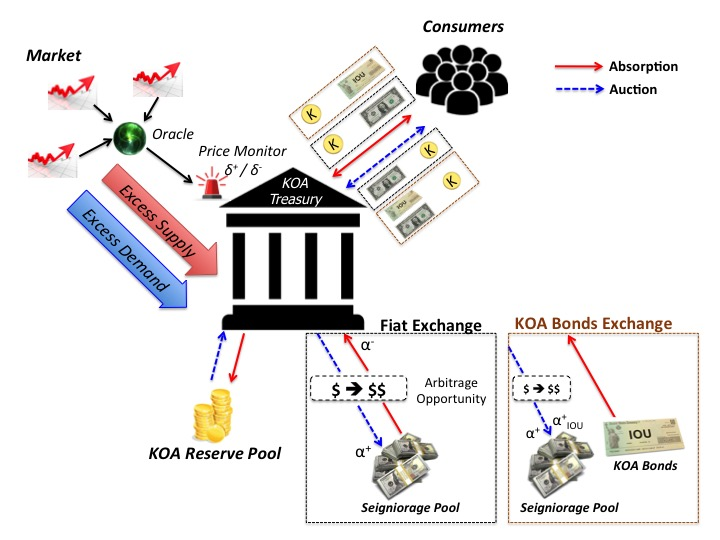
\includegraphics[keepaspectratio, width=0.7\textwidth]{images/treasury.jpg}
    \caption{High Level Overview of the KOA Treasury} \label{fig:treasury}
\end{figure}

\subsubsection{Price and Treasury Dynamics}
The price of KOA is assumed to evolve as a \textit{random walk} when within the target price range and jumps back to the baseline price during tranche periods, as follows
%
\begin{equation} \label{eq:price}
\begin{aligned}
p_{t+1} =
\begin{cases}
      p_t + \xi_t, & p_t \in [p^* - \delta^- p^*, p^* + \delta^+ p^*] \\
      p^*, & \text{otherwise}
\end{cases}
\end{aligned}
\end{equation}
%
where $t \in \{0,...,T\}$ and the $i$-th tranche occurs at time $t_i$. The sequence $\{\xi_t\}$ is \textit{independent} and \textit{identically distributed} (\iid), \ie\ $\xi_t$ $\sim$ \iid\ $(\mu, \sigma^2)$. In order to make this assumption, it is sufficient to pick values of $t$ at which to observe the market price such that price evolutions lack non-randomness and follow the efficient market hypothesis (EMH). Proving EMH justifies the random walk model in Equation \ref{eq:price}. It was found that 1 day price observations of Bitcoin showed a lack of significant non-randomness \textbf{(solver world or just prove this ourselves)}, which is further validated by a study done in \cite{Bartos15}. Hence, the oracle in Figure \ref{fig:treasury} will observe the price of KOA at 1 day intervals. This price measurement will be taken as the average price of the price reported from various market trackers.

In order to analyze the robustness of the KOA treasury, the effects of tranches on the distributed KOA supply, the KOA reserve, and the Seigniorage pool are modeled as follows,
%
\begin{align*}
& \qquad \quad \, Q_{i+1} = Q_i + u_i \\
& \qquad \quad \, R_{i+1} = R_i - u_i \\
& u_i =
\begin{cases}
      Q_i \delta^+,  & p_i = (1+\delta^+)p^* \\
      -Q_i \delta^-,  & p_i = (1-\delta^-)p^*
\end{cases}  \\
S_{i+1} = & \begin{cases}
      S_i + p^*(1+\delta^+)(1-\alpha^+)u_i, & u_i > 0 \\
      S_i - p^*(1 - \delta^-)(1+\alpha^-)u_i, & u_i < 0
\end{cases} 
\end{align*}
%
where $i \in \mathbb{Z}_{>0}$ represent an index for the tranche occurrences during some time period $T$, $Q_i$ represents the supply of KOA in distribution, $R_i$ the balance of KOA in the treasury reserves, and $S_i$ the total amount of fiat in the seigniorage pool during the $i$-th tranche. Also, $u_i$ represents the amount of KOA the treasury auctions or absorbs during the $i$-th tranche where $p_i$ is the price of KOA during the $i$-th tranche. Note that there are several assumptions made in this model. First, it assumes that a $\delta^+$ (or $\delta^-$) change in price will require a $\delta^+$ (or $\delta^-$) change in KOA supply distributed in order to bring the price back to $p^*$. Secondly, the price goes back to baseline instantaneously once the treasury distributed (or absorbs) the required KOA. \textbf{illustration of indexing here}

Now a tranche is initiated whenever the price of KOA ``walks out" of the target price range, increasing or absorbing the supply as required to reconnect to $p^*$. The sequence of \textit{waiting times} $\{ \tau^+_i \}_{i \geq 1}$ that the price, $p_t$, falls above the upper threshold price rate is assumed to be a sequence of independent exponential random variables with mean $\lambda^+$ (termed the \textit{auction rate}). Let $T_n = \sum_{i=0}^n \tau_i^+$  be a random variable that represents the time the price exceeds the upper threshold for the $n$-th time. The number of times the price exceeds $\delta^+$ percent of $p^*$,
%
\begin{equation} \label{eq:bullcount}
N_t = \sum_{n \geq 1} 1_{t \geq T_n} 
\end{equation}
%
is a Poisson process with probability distribution $\mathbb{P}(N_t = n) = e^{-\lambda^+ t} \frac{(\lambda^+ t)^n}{n!}$. The sequence of waiting times $\{ \tau^-_i \}_{i \geq 1}$ that $p_t$ falls below the bottom threshold price rate has similar characteristics but with mean $\lambda^-$ (called the \textit{absorb rate}). The definition of $T_m$ is similar to that of $T_n$, except that it is the time the price drops below the bottom threshold for the $m$-th time. Hence, the number of times the price declines below $\delta^-$ percent of $p^*$ is defined as follows
%
\begin{equation} \label{eq:bearcount}
M_t = \sum_{m \geq 1} 1_{t \geq T_m} 
\end{equation}

\subsubsection{Absorption Tranche}
\jacomment{Now that the treasury is fully characterized, it is now possible to answer the first of the questions posed earlier: how much seigniorage must the pool contain such that it will never be depleted? Given that $R_0$ is chosen to be sufficiently large}{Maybe add $S_{M_t}$ explanation here?}%
%
\footnote{In fact it was discovered in \cite{Ath08} that buffer stock reserves containing a small percentage of the distributed equilibrium supply was sufficient in maintaining price stability. In other words, if the supply is close to the fundamental value (FV) supply, a reserve supply of about $1$-$2$ percent of the FV supply will be able to keep price stable. Setting $R_0$ such that $R_0 >> S_0$, should satisfy this condition as the reserve has more than it needs to allow the initial supply to get to the FV supply and maintain the supply there without running out.} 
%
and that there is not a complete loss in demand, this question can be answered by considering a scenario where prices are monotonically decreasing over some period during T (\ie\ $p_{t+1} \leq p_t \leq ... \leq p_0$). In this situation, the treasury initiates a series of absorption tranches that absorbs a maximum seigniorage amount of $S^*$. 
%
\begin{equation} \label{eq:Smax}
S^* = p^*(1-\delta^-)(1+\alpha^-)Q_0
\end{equation}
%
This is defined as the \textit{Optimal Seigniorage} and follows from Lemma \ref{lemma:Smax} in the appendix.

In other words, the KOA treasury will never deplete its seigniorage pool if it contains at or above $S^*$ prior to a worst case scenario bear market. The problem is that this amount can be fairly large and grows as the distributed KOA supply grows. Collecting the required capital to meet this amount may be impractical and as the seigniorage pool grows, this stabilization scheme runs into similar problems that plague non-collateralized schemes. Hence, it is highly desirable to have a small and efficient, but robust seigniorage pool that will be able to handle a large band of worst-case market scenarios. A treasury that meets this criteria is defined as one with a \textit{Robust-and-Agile} (\textit{RAA}) seigniorage pool. Hence, the next task is to answer the second question posed above: how much seigniorage must the pool contain such that the probability of running out of seigniorage is small?

A \textit{RAA} seigniorage pool, $\hat{S} = \epsilon S^*$ where $\epsilon \in \mathbb{R}_{>0}$ is called the \textit{RAA parameter}, is one that has a lower than 30\% chance of being depleted during some period $T$. Theorem \ref{thm:bearbounds} in the appendix shows that the probability of depleting the treasury during this time is defined as follows.
%
\begin{equation} \label{eq:bearbounds}
\begin{aligned}
& 1 - \Phi (\sign(\log_{1- \delta^-}(1-\epsilon) - \lambda^- +1) \sqrt{(2H(\lambda^-, \log_{1- \delta^-}(1-\epsilon) +1))}) \\
& < \prob(\text{deplete}) \\
& < 1 - \Phi (\sign(\log_{1- \delta^-}(1-\epsilon) - \lambda^-) \sqrt{(2H(\lambda^-, \log_{1- \delta^-}(1-\epsilon)))})
\end{aligned}
\end{equation}
%
where $\sign(\cdot)$ is the signum function and $\Phi(\cdot)$ is the standard normal cumulative distribution function. Given any $S_0$ (as defined by being some $\epsilon$ percent of $S^*$), the probability that it will be depleted during period $T$ can be easily computed by Equation \ref{eq:bearbounds}. Per the definition of a RAA seigniorage pool, $\hat{S}$ is defined as any $\hat{S} = \epsilon S^*$ such that $\prob(M_T \geq  \log_{1- \delta^-}(1-\epsilon)) <$ 0.3.

\subsubsection{Auction Tranche}
Now that the amount of seigniorage required to handle a band of bearish behavior has been determined, the next step is to determine the bull market bull behavior required to replenish the pool and ensure the required seigniorage exists at the beginning of period $T+1$. Consider a scenario where price is monotonically increasing after a bear market and the number of times the price exceeds $\delta^-$ takes on the counting Poisson Process in Equation \ref{eq:bullcount}. The treasury therefore initiates a series of auction tranches causing the seigniorage pool to replenish incrementally as follows.
%
\begin{align*}
\Delta S_i^+ = S_{i+1}^+ - S_i^+ = p^*(1+\delta^+)(1-\alpha^+)u_i 
\end{align*}
%
Again, since $u_i = Q_i\delta^+$ and $\Delta S_i^+ = p^*(1+\delta^+)(1-\alpha^+)Q_0(1-\delta^+)^i\delta^-$ follows, then $S_{N_t}$ denotes the amount of reserves auctioned off during some time $t$ and is defined as
%
\begin{equation} \label{eq:Sreplenish}
S_{N_T} = p^*(1+\delta^+)(1-\alpha^+)Q_0\big((1+\delta^+)^{N_T} - 1 \big)
\end{equation}
%
The objective is to determine the probability that the seigniorage pool will be replenished by a bull market during $T$, \ie\ $\prob(S_{N_T} \geq S_{M_T})$. In order to carry out the analysis, the following \textit{sufficiency assumptions} are made
%
\begin{equation*} \label{eq:sufficientassumptions}
\delta^+ \geq \alpha^-, \quad \delta^- \geq \alpha^+
\end{equation*}
%
These assumptions ensure that $N_T \geq M_T$ is a \textit{sufficient} condition for the $S_{N_T} \geq S_{M_T}$ inequality to hold. Thus, since $N_T \geq M_T$ implies this original inequality, then $\prob(S_{N_T} \geq S_{M_T})$ can be closely approximated by $\prob(N_T \geq M_T)$.

Since $N_T \sim$ Poiss($\lambda^+$) and $M_T \sim$ Poiss($\lambda^-$), where $N_T$ and $M_T$ are independent RVs, $W_T = N_T - M_T$ takes on a \textit{Skellam distribution}, in other words $W_T \sim$ Skellam($\lambda^+ - \lambda^-$, $\lambda^+ + \lambda^-$). The probability of replenishing the treasury can be computed easily as follows
%
\begin{equation} \label{eq:bullbounds}
\prob(\text{replenish}) = \prob(W_T \geq 0) = 1 - \psi(0, \lambda^+, \lambda^-)
\end{equation}
%
where $\prob(\text{replenish}) = \prob(N_T \geq M_T)$ and $\psi(\cdot)$ is the CDF of $W_T$, which has no closed form solution but can easily be numerically computed. The analysis above was conducted for a worst-case  scenario in which the price decreases continuously, but the result applies to the more general case where the price changes non-uniformly throughout some period $T$. 

\subsection{Data and Discussion}

\subsubsection{Finding Auction and Absorb Rates} \label{thresholdDiscussion}
In order to compute the bounds, it is necessary to know the values for $\lambda^+$ and $\lambda^-$. These rates represent the number of times the price exceeds $\delta^+$ or declines below $\delta^-$ of the target price, respectively, in a given period of time. Table \ref{table:avgdata} shows different values of $\lambda^+$ and $\lambda^-$ for various cryptocurrencies at different values of $\delta^+$ or $\delta^-$ between November 1, 2017 to April 1, 2018 (\ie\ $T = 5$ months). During the earlier stages of this period, the cryptocurrency market experienced a large surge in market cap as it thrusted into the media spotlight. Holidays, increasing regulations in Asia, and overvaluation in the earlier months resulted in a steady decrease in price in the latter months of this period. It is possible to observe worst-case volatility behavior by measuring $\lambda^+$ and $\lambda^-$ during periods of high speculation, allowing Equations \ref{eq:bearbounds} and \ref{eq:bullbounds} to yield conservative estimates. Furthermore, these observed values are likely higher than they would be if a price stabilization scheme were in place for each cryptocurrency. Hypothetically, if the market knew the price of a cryptocurrency would be stabilized endogenously, then speculation should be significantly less and price changes should result from changes in true demand. 
% Notes to add throughout
%When determining $\lambda^+$ and $\lambda^-$, it is assumed that the price at each time $t$ (see Equation \ref{eq:price}) is \textit{independent} of the price at any other time and that the bear periods are \textit{independent} of the bull periods (\ie\ $M_t$ is independent of $N_t$). 
%For the first assumption, it is sufficient to pick values of $t$ at which to observe the market price such that a random walk model if valid. It was found that 1 day price observations of Bitcoin showed a lack of significant non-randomness {solver world or just prove this ourselves}, which was further validated by studies {cite "does bitcoin follow hypothesis of efficient market"}. 
%Reference "Price stabilization via Buffer stocks" to justify 100 billion coin supply. Only a fraction of equilibrium supply capacity is required in reserves to stabilize price.

Table \ref{table:avgdata} highlights the relationship between the set threshold rates and their respective absorb and auction rates. It can be seen that for all cases, as the price threshold rates increase the treasury intervenes less to stabilize the price. This is expected since a larger target price range allows the price to evolve and possibly self correct on its own. Thus, Equations \ref{eq:Sdeplete} and \ref{eq:Smax} show that the treasury requires less seigniorage in order to stabilize back to the target price at higher values of $\delta^-$. This is consistent with a finding on exchange rate stabilization using buffer stocks in \cite{Kot08}, in which central banks incur less cost when they attempt to track the exchange rate towards the currency's fundamental value. Similarly, if the target price range increases it will more likely contain KOA's fundamental value ($\tilde{p}$), requiring less intervention from the treasury. The value of $\delta^-$ must be high enough to increase the likelihood of this condition, but not too high where significant amounts of volatility is tolerated. This value will also depend on how far $p^*$ is from KOA's fundamental value (which will depend on the true demand of KOA). The further $p^*$ is from $\tilde{p}$, the greater $\delta^-$ must be in order to maintain the likelihood of $\tilde{p}$ in the target price range. On the other hand, the upper threshold rate can be set to a relatively low value to keep the price close to the target price, while accumulating more seigniorage. How the threshold rates are adjusted and at what value to set $p^*$ will be discussed in a later section. %Talk about this further in the next section
%
\begin{table}[]
\centering
\begin{tabular}{|c|c|c|c|c|c|c|}
\hline
\multicolumn{1}{|l|}{}                                               & \multicolumn{3}{c|}{$\lambda^+$}          & \multicolumn{3}{c|}{$\lambda^-$}       \\ \hline
\multicolumn{1}{|l|}{}                                               & $\delta^+=0.15$  & $\delta^+=0.20$ & $\delta^+=0.30$            & $\delta^-=0.15$  & $\delta^-=0.20$ & $\delta^-=0.30$ \\ \hline
Bitcoin                                                          & $12$ & $8$ & $6$           & $9$  & $6$ & $3$     \\ \hline
Ethereum                                                        & $11$    & $8$    & $5$             & $9$ & $6$ & $3$     \\ \hline
\begin{tabular}[c]{@{}c@{}}Ripple\end{tabular} & $14$    & $13$    & $8$ & $13$        & $10$        & $4$     \\ \hline
\begin{tabular}[c]{@{}c@{}}OmiseGo\end{tabular} & $17$    & $11$    & $6$ & $13$        & $7$        & $3$     \\ \hline
\end{tabular}
\caption{Values of $\lambda^+$ and $\lambda^-$ for Various Cryptocurrencies During a $T = 5$ month period} \label{table:avgdata}
\end{table}

\subsubsection{Robustness of KOA Treasury}

This section discusses the robustness of the KOA treasury and how it is affected by the treasury parameters. Combining the complement of Equation \ref{eq:bearbounds} with \ref{eq:bullbounds} yields bounds on the probability that the treasury will maintain its seigniorage pool during a given period. This is called the treasury's \textit{robustness probability} and is shown below
%
\begin{equation} \label{eq:robustbounds}
\begin{aligned}
& (1-\psi(0, \lambda^+, \lambda^-)) \prob^-(S_{M_T} \geq S_0) \\
& < \prob(\text{robust}) \\
& < (1-\psi(0, \lambda^+, \lambda^-)) \prob^+(S_{M_T} \geq S_0)
\end{aligned}
\end{equation}
%
where $\prob^-(S_{M_t} \geq S_0) = \Phi (\sign(\log_{1- \delta^-}(1-\epsilon) - \lambda^-) \sqrt{(2H(\lambda^-, \log_{1- \delta^-}(1-\epsilon)))})$, $\prob^+(S_{M_t} \geq S_0) = \Phi (\sign(\log_{1- \delta^-}(1-\epsilon) - \lambda^- +1) \sqrt{(2H(\lambda^-, \log_{1- \delta^-}(1-\epsilon) +1))})$, and $\prob(robust) = \prob(S_0 \geq S_{M_T} \cap N_T \geq M_T)$. Note that these bounds depend highly on the treasury's parameters at each period. 

Consider when the treasury maintains a seigniorage pool greater than $S^*$ (\ie\ $S_0 \geq S^*$)-- in this case the treasury has no chance of depleting its seigniorage pool in a given period. The treasury's robustness probability will depend only on its replenish probability, which is the probability that there is greater overall demand in that period (probability of more auctions than absorptions). The threshold rates $\delta^+$ and $\delta^-$ significantly impact this probability due to their relationship with $\lambda^+$ and $\lambda^-$, respectively (see Section \ref{thresholdDiscussion}). The threshold rates should be chosen not only to control a range of volatility, but also so that $\lambda^+ >> \lambda$. It is sufficient to say that values for $\lambda^+$ and $\lambda^-$ such that $\lambda^+ \geq 2 \lambda^-$ meets this condition. In the case where $S_0 \geq S^*$, the robustness of the treasury will depend strictly on the relative values of $\lambda^+$ and $\lambda^-$. Fortunately, due to the cryptocurrency market's (super)-exponential growth in market capitalization (and demand) \cite{ElBahrawy17}, it is expected that $\lambda^+ >> \lambda^-$ for a given $\delta^+$ and $\delta^-$ for $\delta^+ \leq \delta^-$. Hence, the rate at which the KOA treasury collects seigniorage will be greater than the rate that it spends them. Considerations for choosing the threshold rates are discussed further in Section \ref{thresholdDiscussion}.

In the case where the treasury maintains an RAA Seigniorage pool (\ie\ $S_0 = \hat{S}$), the robustness probability will depend on the size of the seigniorage pool and the rate at which demand for KOA decreases. Note that maintaining a smaller seigniorage pool (\ie\ $\epsilon$ is lower) results in a higher probability of it being depleted. As discussed in Section \ref{thresholdDiscussion}, a decrease in $\delta^-$ will result in greater intervention from the treasury (\ie\ increase in $\lambda^-$). This will result in greater depletion of the seigniorage pool, especially if the smaller target price range does not contain KOA's fundamental value. 

\subsection{Choosing the Parameters of the KOA Treasury}
Each parameter in the KOA treasury serves a specific purpose in the overall stabilization scheme. These parameters are set at the beginning of each period $T$ and should be adjusted appropriately to keep the price of KOA stable around the target price. This should be done while maximizing the amount of seigniorage collected during each period. The main challenge is to determine these parameter values \textit{apriori} and in a smart way that achieves the previously stated goals. This is a difficult problem due to the parameters' nonlinear effects on seigniorage and the uncertainty in market behavior. As part of the discussion in the next paragraph, it is assumed that the parameters adhere to the assumptions in Section \ref{eq:sufficientassumptions}.

The parameters of the KOA treasury are its threshold rates, arbitrage rates, RAA parameter, and target price. First, the main purpose of threshold rates $\delta^+$ and $\delta^-$ is to maintain the stability of KOA around the target price. These rates determine the target price range and are used to set the price tolerances on KOA at each time period. Refer to Section \ref{thresholdDiscussion} for a more detailed discussion of threshold rates and their effects on the stabilization scheme. For the purposes of implementation, $\delta^+$ will be initially restricted to be no less than 5\%. This is due to the fact that cryptocurrency prices easily surpass 5\% within a day (or less), hence would result in trivially long periods of auction tranches. \textbf{This could lead to a scenario where too much excess demand is taken from the exchanges, leading to a depreciation in the price of KOA.} Table \ref{table:avgdata} displays a reasonable range of values for setting the threshold rate.

The arbitrage rates serve as parameters to incentivize users to buy and sell KOA from the treasury when the price needs to be corrected back to target price. The objective is to make $\alpha^+$ and $\alpha^-$ sufficiently large in order to pull enough excess demand (supply) from the exchanges such that the price decreases (increases) back to the target price. On the other hand, $\alpha^+$ and $\alpha^-$ should not be so large such that the treasury is depleting seigniorage faster than obtaining it. Reasonable values for arbitrage rates should lie between 5\% and 30\%, depending on several market factors. For example, if the market price of KOA corrects relatively fast (within a few hours), then the treasury should sell KOA at the target price (\ie\ the arbitrage rate is equal to the threshold rate). In this case, setting the arbitrage rate lower than the threshold rate will have no effect on pulling excess demand from the exchanges since market price of KOA will be strictly lower than the treasury price. On the other hand, if the price of KOA corrects very slowly, then the KOA treasury presents users sufficient arbitrage opportunity to incentivize them to buy from the treasury. It is then beneficial to set the arbitrage rate to a value smaller than the threshold rate.

The target price, $p^*$, represents the fiat price to which KOA should be pegged at. This ensures that KOA functions as a unit of account and store of value, making it an effective medium of exchange. Ideally, $p^*$ should be equal to the fundamental value of KOA, $\hat{p}$. Unfortunately, the fundamental value of KOA is difficult to ascertain \textit{apriori} (especially in a speculative economy), hence $p^*$ should be set in the ``neighborhood" of $\hat{p}$. This neighborhood is the target price range and as discussed in Section \ref{thresholdDiscussion}, failing to pick $p^*$ and $\delta^-$ appropriately such that $\hat{p}$ lies in the target price range can lead to excessive intervention from the treasury and thus depletion of the seigniorage pool. For the purpose of implementation, it is assumed that the fundamental value of KOA will be close to the exchange rate of most rewards points to dollars (\eg\ 300 points for every \$1 at La Quinta). Thus, reasonable values for $p^*$ include \$0.002 to \$0.02. 

If the resulting optimal seigniorage ($S^*$) is too large, an RAA parameter $\epsilon$ should be chosen such that the treasury will maintain an RAA seigniorage pool. This parameter ensures the required pool is not too large that it becomes costly to maintain, and so that it is possible to attain the required seigniorage in a reasonable amount of time. Furthermore, $\epsilon$ is chosen appropriately such that the resulting seigniorage pool is minimally likely to be depleted (less than a 30\% chance). This parameter should be computed last after acceptable values for threshold rates, arbitrage rates, and target price have been determined.

\subsection{Proposed Minimum Viable Product}

This section details an initial implementation of the KOA treasury using the planned supply discussed in the ``Token Distribution" section and an estimated target price. Figure \ref{fig:treasury} shows a high level diagram of how the KOA Treasury works.The Koalition protocol will start with an initial distributed supply of $Q_0 = 30$ billion KOA and reserves of $R_0 = 70$ billion KOA. The treasury will attempt to peg the price of KOA to \$0.001, a price that equates to approximately 1000 points per \$1. This first step is to determine appropriate values for the threshold and arbitrage rates. In general, since cryptocurrency behavior is coupled to the market behavior of Bitcoin, the parameters for Bitcoin in Table \ref{table:avgdata} are used to predict KOA's market behavior. Keeping in mind the considerations in the previous section, it is deemed that $\delta^+ = 0.15$ and $\delta^- = 0.30$ not only produce acceptable tolerances for volatility but their associated auction and absorption rates $\lambda^+ = 12$ and $\lambda^- = 3$, respectively, meet the $\lambda^+ >> \lambda^-$ criteria. Next, the arbitrage rates $\alpha^+ = \alpha^- = 0.10$ are chosen to be close to the threshold rates, providing users plenty of arbitrage opportunity in a variety of market conditions where price corrections lag at different rates. Note that these values also fulfill the assumptions set forth in Section \ref{eq:sufficientassumptions}.
%
\begin{table}[]
\centering
 \begin{tabular}{|c | c |} 
 \hline
  $S^*$ & $\$23.1$ million \\ 
 \hline
 $\hat{S}$ $(\epsilon = 0.76)$ & $\$17.6$ million  \\ %epsilon = 0.76
 \hline
 $\prob$(deplete) & $(14.61\%, 29.14\%)$ \\
 \hline
 $\prob$(replenish) & $98.94\%$ \\
 \hline
$\prob$(robust) & $(70.12\%, 84.49\%)$ / $98.94\%$ \\
 \hline
\end{tabular}
\caption{Initial KOA Treasury Seigniorage Pool and Probabilities for $\delta^+ = 0.15$, $\delta^- = 0.30$} \label{table:MVP}
\end{table}

Table \ref{table:MVP} shows the required seigniorages the treasury should maintain and probabilities highlighting the robustness of these respective seigniorage pools. Note that $\prob$(deplete), $\prob$(replenish), and $\prob$(robust) are computed from Equations \ref{eq:bearbounds}, \ref{eq:bullbounds}, and \ref{eq:robustbounds}, respectively. For example, the optimal seigniorage $S^*$ is computed from Equation \ref{eq:Smax} and has robustness probability of $98.94\%$. This means that if the treasury's seigniorage pool was initialized with $S^*$ seigniorage, then the probability of it maintaining its seigniorage throughout a given period is $98.94\%$. On the other hand, if $S^*$ is too large, then an RAA seigniorage pool can be maintained by holding $76\%$ of $S^*$. If an RAA seigniorage pool is maintained, the pool has a probability between $70.12\%$ and $84.49\%$ of holding onto its seigniorage during a given period. While a fiat-collateralized scheme would require the treasury to hold $\$30$ million in collateral to back each value of KOA at $\$0.001$, a non-collateralized scheme maintaining an RAA seigniorage pool requires approximately half that amount.

\subsubsection{KOA Bonds}

As part of the effort to initially build the seigniorage pool, \textit{KOA Bonds} will be issued as a means to absorb the KOA supply. In other words, instead of the treasury buying back KOA, it will offer consumers \textit{bonds} to future KOA at an enticing discount, $\alpha^+_{IOU}$ such that $\alpha^+_{IOU} >> \alpha^+$. How this will work is as follows: when the price drops below the bottom threshold rate, the treasury will initiate an absorb tranche where it will offer KOA bonds to users who are willing to part with their KOA for the promise of a discount in the future. When the price increases above the upper threshold rate, the treasury initiates an auction tranche where it will allow users to redeem their KOA bonds and buy KOA at a discounted rate. The discounted rate, $\alpha^+_{IOU} = \frac{1 - \delta^-}{1+\delta^+}$, equates to the bottom threshold rate price giving users sufficient arbitrage opportunity while allowing the treasury to build its seigniorage pool. Take the following example.
%
\begin{quote}
The price of KOA has dropped from $\$0.001$ to $\$0.0007$. Since the price has dropped below the price threshold, the KOA treasury initiates an absorb tranche. John has 10,000 KOA and decides to trade them all in for 10,000 KOA bonds. The price of KOA stabilizes to within the price range and the absorb tranche ends. Five days later, the price of KOA increases to $\$0.00115$ and the treasury initiates an auction tranche. John redeems his 10,000 KOA bonds and is able to buy 10,000 KOA at a discounted price of $\$0.0007$. John now has $\$11.5$ worth of KOA as opposed to $\$7$ of KOA five days ago while the KOA treasury increases its seigniorage pool by $\$7$.
\end{quote}

In the example above, if John buys KOA on the market at a price \textit{lower} than $\$0.001$ then when the price corrects back to the target price, John will definitely benefit from arbitrage. In the case where John buys KOA on the market for a price \textit{greater} than $\$0.001$, then depending on how fast the market corrects, he may still benefit from arbitrage. If the market corrects to the target price slowly, John will be able to leverage this arbitrage to redeem his KOA at a higher value. Note that the market price will never maintain above $\$0.00115$ since arbitrage from the auction tranches will discourage this behavior. 

%Figure \ref{fig:treasury} shows an overview of how this scheme works. 
% \alpha^+_IOU = 1 - (\delta^+ + \delta^-)/(1+\delta^+)
% Seigniorage shares section
%Speak about fiat exchange versus seigniorage shares. Why it is beneficial to establish fiat exchange in the future
%Seigniorage shares scheme can be used when seigniorage is dangerously low. When is dangerously low?

\subsection{Ongoing Work}

\subsubsection{Seigniorage Shares and Fiat Exchange}

Once the treasury has built an RAA seigniorage pool ($S_0 = \hat{S}$), the original \textit{Fiat exchange} feature will be activated allowing users to redeem their KOA for fiat. The KOA bonds feature will remain, giving users a broader choice of options on how they spend their KOA while maintaining a mechanism for building the seigniorage pool and price stability. \textbf{talk about how this will help incentivize people to redeem their points (absorb)} A \textit{Seigniorage Shares} scheme will also be introduced as an additional stability mechanism to complement the other two. In this scheme users will be able to trade in their KOA for seigniorage shares, entitling them to future seigniorage once the pool is sufficiently replenished. Once enough seigniorage is accumulated, shareholders will be paid an amount strictly higher than that which the treasury would have paid in a fiat exchange. In other words, shareholders will receive $p_{SS} = p^*(1-\delta^-)(1+\alpha^-_{SS})$ per each share, where $\alpha^-_{SS} > \alpha^-$. Furthermore, this scheme acts as an emergency mechanism activated to \textit{replace the fiat exchange} when the seigniorage pool has been excessively depleted during continuous declines in price. Seigniorage shares and KOA bonds will be distributed in an attempt to offset these worst-case market conditions and maintain price stability.

\subsubsection{Increasing Loyalty Through Price Stability}

Price stability has been shown to be a complex problem that involves coordination between Koalition, users, and the market to ensure a thriving ecosystem of points exchange. It is only natural to incorporate loyalty mechanisms in the stability scheme that enables merchants to utilize the Koalition protocol in promoting customer loyalty. For example, KOA can be distributed out to merchants during auction tranches, with the \textit{greatest} KOA distribution volume at a greater discount (greater arbitrage rate). This is effectively a positive feedback loop as it rewards merchants that most utilize the system, giving them more flexibility in rewarding their most loyal customers, and allowing them to distribute more points. During absorb tranches, the most active customers can be given priority in redeeming their KOA for bonds/shares or fiat, effectively rewarding the most active and loyal customers by encouraging redemption of their KOA. Through these features, KOA price stability can unlock new opportunities in the loyalty programs space not possible in legacy loyalty programs. Thus, the future of Koalition and next generation loyalty programs are bright.